\documentclass[11pt,a4paper,oneside]{report}
\usepackage{amsmath,amssymb,calc,ifthen}
\usepackage{float}
%\usepackage{cancel}
\usepackage[table,usenames,dvipsnames]{xcolor} % for coloured cells in tables
\usepackage{tikz}
% Allows us to click on links and references!
\usepackage{hyperref}
\usepackage{url}
\hypersetup{
colorlinks,
citecolor=black,
filecolor=black,
linkcolor=black,
urlcolor=black
}
% Nice package for plotting graphs
% See excellent guide:
% http://www.tug.org/TUGboat/tb31-1/tb97wright-pgfplots.pdf
\usetikzlibrary{plotmarks}
\usepackage{amsmath,graphicx}
\usepackage{epstopdf}
\usepackage{caption}
\usepackage{bbm}
\usepackage{subcaption}
% highlight - useful for TODOs and similar
\usepackage{color}
\newcommand{\hilight}[1]{\colorbox{yellow}{#1}}
\newcommand\ci{\perp\!\!\!\perp} % perpendicular sign
\newcommand*\rfrac[2]{{}^{#1}\!/_{#2}} % diagonal fraction
\newcommand\SLASH{\char`\\}
\usepackage{listings}
% margin size
\usepackage[margin=1in]{geometry}
\tikzstyle{state}=[circle,thick,draw=black, align=center, minimum size=2.1cm,
inner sep=0]
\tikzstyle{vertex}=[circle,thick,draw=black]
\tikzstyle{terminal}=[rectangle,thick,draw=black]
\tikzstyle{edge} = [draw,thick]
\tikzstyle{lo} = [edge,dotted]
\tikzstyle{hi} = [edge]
\tikzstyle{trans} = [edge,->]
\definecolor{mygreen}{rgb}{0,0.6,0}
\definecolor{mygray}{rgb}{0.5,0.5,0.5}
\definecolor{mymauve}{rgb}{0.58,0,0.82}
\DeclareMathOperator*{\argmin}{arg\,min}
\DeclareMathOperator*{\argmax}{arg\,max}
\newcommand*{\Comb}[2]{{}^{#1}C_{#2}}
\lstset{ %
backgroundcolor=\color{white}, % choose the background color; you must add
%\usepackage{color} or \usepackage{xcolor}
basicstyle=\footnotesize, % the size of the fonts that are used for the
%code
breakatwhitespace=false, % sets if automatic breaks should only happen
%at whitespace
breaklines=true, % sets automatic line breaking
captionpos=b, % sets the caption-position to bottom
commentstyle=\color{mygreen}, % comment style
deletekeywords={...}, % if you want to delete keywords from the
%given language
escapeinside={\%*}{*)}, % if you want to add LaTeX within your code
extendedchars=true, % lets you use non-ASCII characters; for
%8-bits encodings only, does not work with UTF-8
frame=single, % adds a frame around the code
keepspaces=true, % keeps spaces in text, useful for keeping
%indentation of code (possibly needs columns=flexible)
keywordstyle=\color{blue}, % keyword style
language=Octave, % the language of the code
morekeywords={*,...}, % if you want to add more keywords to the set
numbers=left, % where to put the line-numbers; possible
%values are (none, left, right)
numbersep=5pt, % how far the line-numbers are from the code
numberstyle=\tiny\color{mygray}, % the style that is used for the line-numbers
rulecolor=\color{black}, % if not set, the frame-color may be changed
%on line-breaks within not-black text (e.g. comments (green here))
showspaces=false, % show spaces everywhere adding particular
%underscores; it overrides 'showstringspaces'
showstringspaces=false, % underline spaces within strings only
showtabs=false, % show tabs within strings adding particular
%underscores
stepnumber=2, % the step between two line-numbers. If it's
%1, each line will be numbered
stringstyle=\color{mymauve}, % string literal style
tabsize=2, % sets default tabsize to 2 spaces
title=\lstname % show the filename of files included with
%\lstinputlisting; also try caption instead of title
}
\title{Graphical Models Coursework 4}
\author{
Razvan Valentin Marinescu\\
Student Number: 14060166\\
\texttt{razvan.marinescu.14@ucl.ac.uk}
\and
Konstantinos Georgiadis\\
Student Number: 14110861\\
\texttt{konstantinos.georgiadis.14@ucl.ac.uk}
}
\begin{document}
\belowdisplayskip=12pt plus 3pt minus 9pt
\belowdisplayshortskip=7pt plus 3pt minus 4pt
\maketitle{}

\section*{Exercise 12.2}

We want to solve the following optimization problem:

$$w^\ast=\argmax_{w}p(y_{1:T}|\mathbf{x}_{1:T},\mathbf{w})$$

We rewrite the optimization problem in the following way:

\begin{align*}
\mathbf{w}^\ast&=\argmax_{w}p(y_{1:T}|\mathbf{x}_{1:T},\mathbf{w})\\
&=\argmax_{\mathbf{w}}\prod_{t=2}^T\frac{1}{\sqrt{2\pi}\sigma_t}e^{-\frac{(y_t-\mathbf{w}^\top\mathbf{x}_{t-1})^2}{2\sigma_t^2}}\\
&\text{The normalization denominators are constants which do not change the solution:}\\
&=\argmax_{\mathbf{w}}\prod_{t=2}^Te^{-\frac{(y_t-\mathbf{w}^\top\mathbf{x}_{t-1})^2}{2\sigma_t^2}}\\
&\text{We can also take the log of the function:}\\
&=\argmax_{\mathbf{w}}\log\left(\prod_{t=2}^Te^{-\frac{(y_t-\mathbf{w}^\top\mathbf{x}_{t-1})^2}{2\sigma_t^2}}\right)\\
&=\argmax_{\mathbf{w}}\log\left(e^{\sum_{t=2}^T-\frac{(y_t-\mathbf{w}^\top\mathbf{x}_{t-1})^2}{2\sigma_t^2}}\right)\\
&=\argmax_{\mathbf{w}}\sum_{t=2}^T-\frac{(y_t-\mathbf{w}^\top\mathbf{x}_{t-1})^2}{2\sigma_t^2}\\
&\text{We can remove the 1/2 factors and the minus signs by changing it into an argmin:}\\
&=\argmin_{\mathbf{w}}\sum_{t=2}^T\frac{(y_t-\mathbf{w}^\top\mathbf{x}_{t-1})^2}{\sigma_t^2}\\
&=\argmin_{\mathbf{w}}\sum_{t=2}^T\left(\frac{y_t}{\sigma_t}-\frac{\mathbf{w}^\top\mathbf{x}_{t-1}}{\sigma_t}\right)^2\\
&\text{We can rewrite this as a least squares problem as such:}\\
&=\argmin_{\mathbf{w}}||\mathbf{X}\mathbf{w}-\mathbf{y}||_2^2\text{, where: }\mathbf{X}=\left[ { \begin{array}{c} \mathbf{x}_1^\top/\sigma_2\\ ... \\ \mathbf{x}_{T-1}^\top/\sigma_T  \end{array} } \right], \mathbf{y}=\left[ { \begin{array}{c} y_2/\sigma_2\\ ... \\ y_{T}/\sigma_T  \end{array} } \right]\\
&\text{The common solution to which, is well known as the following:}\\
\mathbf{w}^\ast&=(\mathbf{X}^\top\mathbf{X})^{-1}\mathbf{X}^\top\mathbf{y}
\end{align*}

The hierarchical belief network is the following:

	\begin{center} 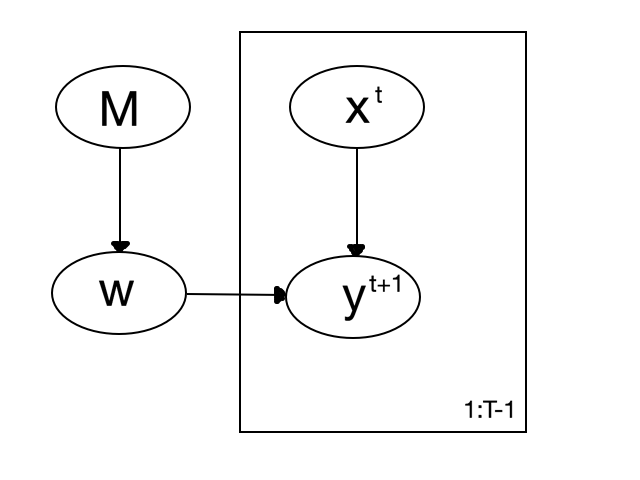
\includegraphics[width=0.5\textwidth]{c12e2beliefnetwork}\end{center}

We initially start with equation 12.4.5:

$$p(M|\mathbf{x}_{1:T-1},\mathbf{y}_{2:T})=\frac{p(\mathbf{x}_{1:T-1},\mathbf{y}_{2:T}|M)p(M)}{p(\mathbf{x}_{1:T-1},\mathbf{y}_{2:T})}$$

The idea is to calculate the above probability for every different model M and then we will choose the one with the highest probability. Let us take for example two of them:

$$\frac{p(M=i|\mathbf{x}_{1:T-1},\mathbf{y}_{2:T})}{p(M=j|\mathbf{x}_{1:T-1},\mathbf{y}_{2:T})}=\frac{\frac{p(\mathbf{x}_{1:T-1},\mathbf{y}_{2:T}|M=i)p(M=i)}{p(\mathbf{x}_{1:T-1},\mathbf{y}_{2:T})}}{\frac{p(\mathbf{x}_{1:T-1},\mathbf{y}_{2:T}|M=j)p(M=j)}{p(\mathbf{x}_{1:T-1},\mathbf{y}_{2:T})}}=\frac{p(\mathbf{x}_{1:T-1},\mathbf{y}_{2:T}|M=i)p(M=i)}{p(\mathbf{x}_{1:T-1},\mathbf{y}_{2:T}|M=j)p(M=j)}$$

However, we are given that the prior p(M) is flat, therefore we need only:

$$\frac{p(M=i|\mathbf{x}_{1:T-1},\mathbf{y}_{2:T})}{p(M=j|\mathbf{x}_{1:T-1},\mathbf{y}_{2:T})}=\frac{p(\mathbf{x}_{1:T-1},\mathbf{y}_{2:T}|M=i)}{p(\mathbf{x}_{1:T-1},\mathbf{y}_{2:T}|M=j)}=\frac{\prod_{t=1}^{T-1}p(x_t)p(\mathbf{y}_{2:T}|\mathbf{x}_{1:T-1},M=i)}{\prod_{t=1}^{T-1}p(x_t)p(\mathbf{y}_{2:T}|\mathbf{x}_{1:T-1},M=j)}$$

By adjusting equation 12.4.6 we are now left with:

$$\frac{p(M=i|\mathbf{x}_{1:T-1},\mathbf{y}_{2:T})}{p(M=j|\mathbf{x}_{1:T-1},\mathbf{y}_{2:T})}=\frac{p(\mathbf{y}_{2:T}|\mathbf{x}_{1:T-1},M=i)}{p(\mathbf{y}_{2:T}|\mathbf{x}_{1:T-1},M=j)}=\frac{\int_{\mathbf{w}}p(\mathbf{w}|M=i) \prod_{t=1}^{T-1}p(\mathbf{y}_{t+1}|\mathbf{x}_t,\mathbf{w},M=i)}{\int_{\mathbf{w}}p(\mathbf{w}|M=j) \prod_{t=1}^{T-1}p(\mathbf{y}_{t+1}|\mathbf{x}_t,\mathbf{w},M=j)}$$

Since we are only interested in model comparison, we can equivalently use equation 12.4.7, after adjusting it to our current problem(we set $\alpha = 1$ right away and $\phi(x_t)=x_t$):

$$2\log p(\mathbf{y}_{2:T}|\mathbf{x}_{1:T-1},M=i)=-\left(\sum_{t=2}^{T}\log \left(2\pi\sigma_t^2\right)+\frac{y_t^2}{\sigma_t^2}\right)+\mathbf{b}^\top\mathbf{A}^{-1}\mathbf{b}-\log \det (\mathbf{A})$$

where:

$$\mathbf{A}=\mathbf{I}+\sum_{t=1}^{T-1}\frac{1}{\sigma_{t+1}^2}\mathbf{x}_t\mathbf{x}_t^\top, \mathbf{b}=\sum_{t=1}^{T-1}\frac{1}{\sigma_{t+1}^2}y_{t+1}\mathbf{x}_t$$

We also note that the first term is not affected by the model choice and therefore is not required in the computation. Therefore, we only need to calculate for each model the following and then find the maximum value:

$$\mathbf{b}^\top\mathbf{A}^{-1}\mathbf{b}-\log \det (\mathbf{A})$$

The MATLAB code used:

\begin{lstlisting}
clear all; clc; close all;
import brml.*
load('dodder.mat');
ModelLikelihoods = zeros(2^6-1,1);
for M = 1:2^6-1
    binary = logical(de2bi(M,6));
    A = eye(sum(binary));
    b = zeros(sum(binary),1);
    for t = 1:T
        A = A + (x(binary,t)*x(binary,t)')/(sigma(t)^2);
        b = b + (y(t)*x(binary,t))/(sigma(t)^2);
        %ModelLikelihoods(M) = ModelLikelihoods(M) + log(2*pi*sigma(t)^2) + (y(t)^2)/(sigma(t)^2);
    end
    ModelLikelihoods(M) = - ModelLikelihoods(M) + b'*(A\b)-log(det(A));
end
[~,BestModel] = max(ModelLikelihoods);
de2bi(BestModel,6)
\end{lstlisting}

MATLAB prints out that the best model is the one using all six of the variables:

ans =

     1     1     1     1     1     1

\section*{Exercise 12.3}

We want to show that:

$$\frac{1}{(2\pi \alpha^{-1})^{K/2}}e^{-\frac{\alpha}{2}\mathbf{w}^\top \mathbf{w}}\frac{1}{(2\pi \sigma^{2})^{N/2}}e^{-\frac{1}{2\sigma^2}\sum_n (y^n-\mathbf{w}^\top \phi(x^n))^2}=\frac{1}{(2\pi \alpha^{-1})^{K/2}}\frac{1}{(2\pi \sigma^{2})^{N/2}}e^{-\frac{1}{2\sigma^2}\sum_n(y^n)^2}e^{-\frac{1}{2}\mathbf{w}^\top\mathbf{A}\mathbf{w}+\mathbf{b}^\top\mathbf{w}}$$

By continual equivalences we have:
\fontsize{10pt}{10pt}\selectfont
\begin{align*}
\text{Removing the fractions:}&\\
e^{-\frac{\alpha}{2}\mathbf{w}^\top \mathbf{w}}e^{-\frac{1}{2\sigma^2}\sum_n (y^n-\mathbf{w}^\top \phi(x^n))^2}&=e^{-\frac{1}{2\sigma^2}\sum_n(y^n)^2}e^{-\frac{1}{2}\mathbf{w}^\top\mathbf{A}\mathbf{w}+\mathbf{b}^\top\mathbf{w}}\\
\text{Taking the logarithm:}&\\
-\frac{\alpha}{2}\mathbf{w}^\top \mathbf{w}-\frac{1}{2\sigma^2}\sum_n (y^n-\mathbf{w}^\top \phi(x^n))^2&=-\frac{1}{2\sigma^2}\sum_n(y^n)^2-\frac{1}{2}\mathbf{w}^\top\mathbf{A}\mathbf{w}+\mathbf{b}^\top\mathbf{w}\\
\text{Expanding the quadratic:}&\\
-\frac{\alpha}{2}\mathbf{w}^\top \mathbf{w}-\frac{1}{2\sigma^2}\left(\sum_n (y^n)^2-2y^n\mathbf{w}^\top\phi(x^n)+(\mathbf{w}^\top\phi(x^n))^2\right)&=-\frac{1}{2\sigma^2}\sum_n(y^n)^2-\frac{1}{2}\mathbf{w}^\top\mathbf{A}\mathbf{w}+\mathbf{b}^\top\mathbf{w}\\
\text{Distributing the sum and rearranging:}&\\
-\frac{\alpha}{2}\mathbf{w}^\top \mathbf{w}-\frac{1}{2\sigma^2}\sum_n (y^n)^2+\frac{1}{\sigma^2}\sum_ny^n\mathbf{w}^\top\phi(x^n)-\frac{1}{2\sigma^2}\sum_n(\mathbf{w}^\top\phi(x^n)\mathbf{w}^\top\phi(x^n))&=-\frac{1}{2\sigma^2}\sum_n(y^n)^2-\frac{1}{2}\mathbf{w}^\top\mathbf{A}\mathbf{w}+\mathbf{b}^\top\mathbf{w}\\
\text{Removing the sum over y's and rearranging:}&\\
-\frac{\alpha}{2}\mathbf{w}^\top \mathbf{I} \mathbf{w}+\mathbf{w}^\top\frac{1}{\sigma^2}\sum_ny^n\phi(x^n)-\mathbf{w}^\top\frac{1}{2\sigma^2}\sum_n(\phi(x^n)\phi(x^n)^\top)\mathbf{w}&=-\frac{1}{2}\mathbf{w}^\top\mathbf{A}\mathbf{w}+\mathbf{b}^\top\mathbf{w}\\
\text{Substituting with the definition of b and rearranging:}&\\
-\frac{1}{2}\mathbf{w}^\top\left(\alpha \mathbf{I} + \frac{1}{\sigma^2}\sum_n\phi(x^n)\phi(x^n)^\top \right) \mathbf{w}+\mathbf{w}^\top\mathbf{b}&=-\frac{1}{2}\mathbf{w}^\top\mathbf{A}\mathbf{w}+\mathbf{b}^\top\mathbf{w}\\
\text{Substituting with the definition of A and rearranging:}&\\
-\frac{1}{2}\mathbf{w}^\top\mathbf{A} \mathbf{w}+\mathbf{w}^\top\mathbf{b}&=-\frac{1}{2}\mathbf{w}^\top\mathbf{A}\mathbf{w}+\mathbf{w}^\top\mathbf{b}\\
\end{align*}

\section*{Exercise 23.4}
\section*{Exercise 23.11}
\section*{Exercise 27.5}
\section*{Exercise 27.6}
\section*{Exercise 27.9}



\end{document}





















